%-------------------------------------------------
% FileName: chapt-1.tex
% Author: Safin (zhaoqid@zsc.edu.cn)
% Version: 0.1
% Date: 2020-05-12
% Description: 第1章
% Others: 
% History: origin
%------------------------------------------------- 

% 断页
\clearpage
% 页码从1开始计数
\setcounter{page}{1}
% 阿拉伯数字显示页码
\pagenumbering{arabic}

\chapter{绪论}

\section{研究背景}
芯片被誉为现代工业的掌上明珠,是信息时代的基石。自1959年世界上第一颗芯片诞生以来\cite{faggin1996history},芯片技术以惊人的速度发展,推动了从个人计算机到智能手机、从数据中心到物联网设备的全面革新。半导体行业也因此成为当今世界最具战略意义和经济价值的行业之一。经过半个多世纪的发展,全球处理器架构市场逐渐形成了两大主流阵营:面向高性能计算的X86架构和面向嵌入式系统的ARM架构。然而,随着技术的不断演进和应用场景的多样化,现有的体系结构逐渐暴露出诸多问题:

\begin{enumerate}[label={\arabic*)},itemsep=0pt, parsep=0pt]
	\item \textbf{复杂指令集架构(CISC)的效率问题}:以X86为代表的复杂指令集架构虽然功能强大,但其指令集冗长且复杂,导致指令执行效率较低。为了实现复杂的指令功能,处理器需要集成更多的晶体管和电路,这不仅增加了芯片的设计难度和制造成本,还显著提高了功耗和发热量,限制了其在低功耗场景中的应用。
	\item \textbf{闭源与授权限制}:X86和ARM架构均属于闭源架构,其核心技术和指令集受到严格的版权保护。使用这些架构需要获得相应公司的授权许可,这不仅增加了研发成本,还限制了中小企业和新兴市场的准入,阻碍了技术的普及和创新。
	\item \textbf{市场垄断与供应商锁定}:由于X86和ARM架构在各自领域的主导地位,相关技术的使用高度依赖于特定供应商的支持。这种市场垄断和供应商锁定的局面导致技术更新缓慢,用户选择受限,进一步抑制了行业的发展活力。
\end{enumerate}

为了解决现有体系结构存在的问题,并顺应现代计算机体系结构设计的发展趋势,RISC-V(开源精简指令集架构)应运而生。RISC-V以其开源、免费、开放和自由的特性,迅速成为全球学术界和工业界关注的焦点。任何个人或组织都可以自由使用、修改和分发RISC-V的设计,这为处理器架构的创新和普及提供了前所未有的机会。

RISC-V的起源可以追溯到20世纪80年代初,当时加州大学伯克利分校的David Patterson教授和斯坦福大学的John Hennessy教授分别提出了精简指令集计算(RISC)理念\cite{cocke1990evolution}。RISC的核心思想是通过简化指令集,使处理器设计更加高效、易于实现和优化。基于这一理念,伯克利分校开发了RISC-I和RISC-II原型机,成功验证了RISC架构的可行性和优越性。2010年,加州大学伯克利分校的Krste Asanović教授及其团队启动了RISC-V项目,旨在设计一种全新的、开放的指令集架构,以满足现代计算的多样化需求\cite{waterman2011risc}。2014年,伯克利团队发布了RISC-V的初始规范,包括32位和64位的基本指令集\cite{asanovic2014instruction},这一规范的发布标志着RISC-V正式进入公众视野。

2015年,RISC-V基金会(RISC-V Foundation)正式成立,吸引了包括谷歌、英特尔、英伟达等全球顶尖科技公司以及众多学术机构和研究组织的加入。2017年,首批基于RISC-V的商用芯片发布,展现了RISC-V在实际应用中的巨大潜力。2020年,为了避免潜在的政治和法律风险,RISC-V基金会迁至瑞士,并更名为RISC-V International,进一步提升了RISC-V的国际化水平和开放性。

如今,RISC-V已成为全球范围内最具活力的开源指令集架构之一,其应用领域涵盖嵌入式系统、物联网、高性能计算、人工智能、数据中心等多个领域。RISC-V的崛起不仅为处理器架构的设计和实现提供了新的思路,也为全球半导体行业注入了新的活力,推动了技术的民主化和创新生态的繁荣发展。

更重要的是,在中国的芯片产业中,主流CPU架构一直受西方国家的制约,整体的处理器行业生态与国际先进水平依旧存在不小的差距,RISC-V架构的出现为中国开源芯片的发展提供了新的机遇。2021年,开源首次被写入《中华人民共和国国民经济和社会发展第十四个五年规划和2035年远景目标纲要》\cite{JJRB202112060060},全国各界都投入到对RISC-V开源生态的建设,对RISC-V的支持大幅度上升。例如,由多家RISC-V领域重点企业、研究机构、行业协会发起成立的``中国RISC-V产业联盟'';由网信办、中科院等多个国家部委支持成立的``中国开放指令生态RISC-V联盟'';由加州伯克利大学和清华大学合作发起成立的``RISC-V国际开源实验室'';由中科院、多家行业龙头企业和顶尖科研单位发起成立的``北京开源芯片研究院''等。以上例子说明在国家的政策支持下,各行各业的积极参与下,中国的RISC-V开源生态环境正在以不可阻挡的速度发展。


\section{国内外研究现状}
近年来,RISC-V技术以其开源、模块化和可扩展的特性,在全球范围内引发了广泛关注,并取得了令人瞩目的研究成果。从高性能计算到嵌入式系统,从学术研究到商业应用,RISC-V正在迅速崛起,成为处理器架构领域的重要力量。

2019年,西部数据公司(Western Digital)推出了SweRV核心,这是一款高性能的RISC-V处理器核心,专为数据中心和存储应用设计,SweRV的发布不仅展示了RISC-V在高性能计算领域的潜力,还标志着RISC-V从学术研究向工业应用的重大跨越\cite{marena2019risc}。2021年,阿里巴巴旗下的平头哥半导体发布了玄铁907处理器,这是一款基于RISC-V架构的高性能处理器,已成功授权给多家企业使用,进一步推动了RISC-V的商业化进程\cite{JCDI202106005}。2024年,中国科学院计算技术研究所推出了``香山''昆明湖架构V2,这是一款开源的高性能RISC-V处理器,其卓越的性能和创新的设计再次证明了RISC-V在技术创新上的巨大潜力\cite{JFYZ202303014}。

在系统级集成方面,Vedran Dakić等人提出了一种异构RISC-V SoC设计,该设计集成了高性能的乱序核心、高能效的顺序核心以及专用加速器,充分展现了RISC-V在灵活性和可扩展性方面的优势\cite{electronics13173494}。此外,Koch等人开发了针对RISC-V的FPGA框架FABulous,为RISC-V处理器的快速原型设计和验证提供了高效的工具支持\cite{10.1145/3431920}。在低功耗设计方面,邓等人设计了一款超低功耗RISC-V流水线结构处理器,适用于物联网等低功耗场景\cite{DZJY201906011}。在设计方法学方面,钟等人提出了一种软硬件联合验证的设计方法,通过结合Verilator软件仿真和FPGA硬件验证,显著提高了RISC-V处理器的开发效率和可靠性\cite{SDDZ202411008}。在总线设计方面,郝等人采用ARM公司提出的AHB总线协议,成功实现了系统总线的设计,不仅保持了处理器的高性能,还显著减小了芯片的流片面积\cite{JSGG202020007}。针对浮点数运算的挑战,潘等人提出了一种优化的浮点运算单元(FPU)设计,通过改进算法和硬件结构,显著提升了浮点数运算的效率和精度\cite{JSGG202103009}。

\section{技术对比}
在现代处理器架构中,RISC(精简指令集计算)和CISC(复杂指令集计算)是两种主要的设计理念。以RISC-V、X86和ARM为例,RISC-V作为RISC架构的代表,展现出显著的优势,尤其是在开源性、模块化设计、可扩展性、功耗和性能等方面。

\begin{enumerate}[label={\arabic*)},itemsep=0pt, parsep=0pt]
	\item 在开源性方面,RISC-V的完全开源特性使其在灵活性和可扩展性方面远超X86和ARM。这种开源性不仅降低了开发成本,还允许开发者根据具体需求进行定制和优化,从而推动了创新和多样化应用的开发。相比之下,X86和ARM均为非开源架构,需要授权才能使用,这在一定程度上限制了其在特定领域的应用。

	\item 在处理器设计方面,RISC-V的模块化设计和高可扩展性是其显著优势。它允许开发者根据不同的应用场景灵活选择和扩展指令集,从而更好地适应从嵌入式系统到高性能计算的多样化需求。而X86架构由于其复杂指令集和非模块化设计,在可扩展性方面表现较差,难以满足新兴应用的快速变化需求。

	\item 在功耗方面,RISC-V的设计理念使其在低功耗场景中表现出色。其简洁的指令集和高效的执行效率使得处理器能够在较低的功耗下运行,这对于移动设备和物联网应用尤为重要。相比之下,X86架构由于其复杂的设计和较高的功耗,在移动和嵌入式领域存在明显劣势,尽管其在高性能计算中仍具有一定的优势。

	\item 在性能方面,RISC-V通过高效的指令执行和流水线设计,能够实现高性能处理。虽然X86和ARM在某些应用场景中也能提供高性能,但RISC-V的高效设计使其在功耗和性能的平衡上更具优势。此外,RISC-V的开源性和模块化设计进一步增强了其在性能优化方面的潜力。

	\item 在指令数量方面,与 X86 架构的指令集相比,RISC-V 的指令集格式更为简洁且高效。RISC-V 仅定义了六种指令格式,且每条指令长度固定为 32 位或 64 位,这极大地降低了指令译码时的复杂度和开销。相比之下,X86 架构由于其CISC的特性,指令长度不定,每次取指需按照最大指令字长读取,并在译码阶段进行分割,这无疑增加了指令处理的复杂度。此外,RV32I 的基础指令数量仅为 47 条,即使加上乘除法扩展(RV32M),指令总数也不超过 60 条。如图\ref{fig:x86_growth}所示, X86 架构在发布初期有 80 条指令,到 2015 年,其指令数量已增长至 1338 条,增加了 16 倍。

	      \begin{figure}[htbp]
		      \centering
		      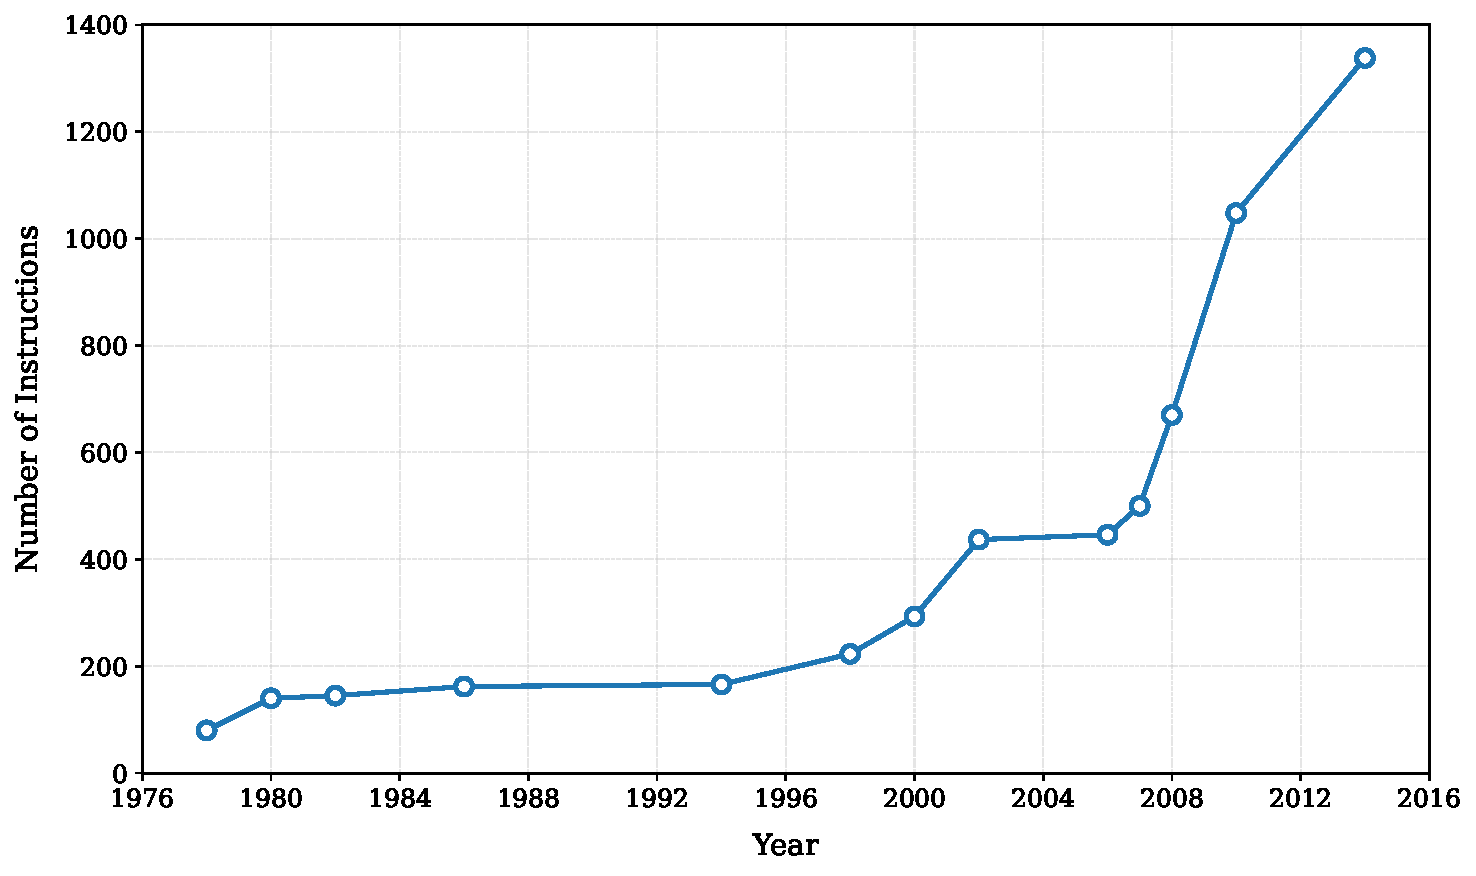
\includegraphics[width=0.8\textwidth]{image/x86_growth.pdf}
		      \caption{x86指令集发展历程(1978-2014)}
		      \label{fig:x86_growth}
	      \end{figure}

\end{enumerate}

综上所述,RISC-V作为RISC架构的代表,在开源性、模块化设计、可扩展性、功耗和性能等方面展现出显著的优势,使其在现代处理器架构中具有广阔的应用前景。

\begin{table}[htbp]
	\centering
	\caption{指令集对比}
	\begin{tabularx}{\textwidth}{>{\centering\arraybackslash}X >{\centering\arraybackslash}X >{\centering\arraybackslash}X >{\centering\arraybackslash}X}
		\toprule
		\textbf{特性} & \textbf{RISC-V} & \textbf{X86} & \textbf{ARM} \\
		\midrule
		类型          & RISC            & CISC         & RISC         \\
		开源性         & 开源              & 闭源           & 闭源           \\
		模块化         & 支持              & 不支持          & 不支持          \\
		扩展性         & 高               & 低            & 低            \\
		功耗          & 低               & 高            & 低            \\
		性能          & 高               & 高            & 高            \\
		\bottomrule
	\end{tabularx}
	\label{tab:instruction-set-comparison}
\end{table}

\section{本章小结}
本章从研究背景、国内外研究现状以及技术对比三个方面对RISC-V架构进行了全面介绍。首先,通过对现有处理器架构(如X86和ARM)的分析,指出了复杂指令集架构(CISC)的效率问题、闭源与授权限制以及市场垄断与供应商锁定等问题。这些问题的存在促使了开源精简指令集架构(RISC-V)的诞生。RISC-V以其开源、免费、开放和自由的特性,迅速成为全球学术界和工业界关注的焦点,为处理器架构的创新和普及提供了前所未有的机会。

在国内外研究现状方面,近年来RISC-V技术取得了显著的进展。从嵌入式系统到高性能计算,从学术研究到商业应用,RISC-V正在迅速崛起,成为处理器架构领域的重要力量。众多企业和研究机构纷纷推出了基于RISC-V的处理器和相关技术,进一步推动了RISC-V的商业化进程和技术创新。

在技术对比部分,通过对RISC-V、X86和ARM三种架构的详细对比,展示了RISC-V在开源性、模块化设计、可扩展性、功耗和性能等方面的优势。RISC-V的完全开源特性降低了开发成本,其模块化设计和高可扩展性使其能够灵活适应多样化的应用场景。在功耗方面,RISC-V的设计理念使其在低功耗场景中表现出色,而其高效的指令执行和流水线设计则使其在性能上具有显著优势。

总的来说,RISC-V具有极高的发展潜力,且逐渐成为X86和ARM双足鼎立之后的``第三极''。